\documentclass[11pt]{article}

\usepackage{graphicx}
\usepackage{geometry}
\usepackage[inline]{enumitem}
\usepackage{moreenum}
\usepackage{xcolor}
\usepackage[bookmarks]{hyperref}
\usepackage[font=small]{caption}
\usepackage{siunitx}
\usepackage{multirow}

\hypersetup{
	colorlinks=true,
	linkcolor=red,
	urlcolor=green,
	filecolor=cyan,
	citecolor=purple,
}

\title{Plato's Life}
\author{Tejas Sanap}
\date{\today}

\begin{document}
	\maketitle
	\tableofcontents

	\section{Introduction}
		% fix quotes and ---
		% Plato (429?–347 B.C.E.) is, by any reckoning, one of the most dazzling writers in the Western literary tradition and one of the most penetrating, wide-ranging, and influential authors in the history of philosophy. An Athenian citizen of high status, he displays in his works his absorption in the political events and intellectual movements of his time, but the questions he raises are so profound and the strategies he uses for tackling them so richly suggestive and provocative that educated readers of nearly every period have in some way been influenced by him, and in practically every age there have been philosophers who count themselves Platonists in some important respects. He was not the first thinker or writer to whom the word “philosopher” should be applied. But he was so self-conscious about how philosophy should be conceived, and what its scope and ambitions properly are, and he so transformed the intellectual currents with which he grappled, that the subject of philosophy, as it is often conceived—a rigorous and systematic examination of ethical, political, metaphysical, and epistemological issues, armed with a distinctive method—can be called his invention. Few other authors in the history of Western philosophy approximate him in depth and range: perhaps only Aristotle (who studied with him), Aquinas, and Kant would be generally agreed to be of the same rank.

		Plato (429?–347 B.C.E.) is, by any reckoning, one of the most dazzling writers in the Western literary tradition and one of the most penetrating, wide-ranging, and influential authors in the history of philosophy. An Athenian citizen of high status, he displays in his works his absorption in the political events and intellectual movements of his time, but the questions he raises are so profound and the strategies he uses for tackling them so richly suggestive and provocative that educated readers of nearly every period have in some way been influenced by him, and in practically every age there have been philosophers who count themselves Platonists in some important respects. He was not the first thinker or writer to whom the word ``philosopher" should be applied. But he was so self-conscious about how philosophy should be conceived, and what its scope and ambitions properly are, and he so transformed the intellectual currents with which he grappled, that the subject of philosophy, as it is often conceived --- a rigorous and systematic examination of ethical, political, metaphysical, and epistemological issues, armed with a distinctive method --- can be called his invention. Few other authors in the history of Western philosophy approximate him in depth and range: perhaps only Aristotle (who studied with him), Aquinas, and Kant would be generally agreed to be of the same rank.

		 Like most other ancient philosophers, Plato maintains a virtue-based eudaemonistic conception of ethics. That is to say, happiness or well-being (eudaimonia) is the highest aim of moral thought and conduct, and the virtues (aretê: `excellence') are the requisite skills and dispositions needed to attain it. If Plato's conception of happiness is elusive and his support for a morality of happiness seems somewhat subdued, there are several reasons. First, he nowhere defines the concept or makes it the direct target of investigation, but introduces it in an oblique way in the pursuit of other questions. Second, the treatment of the human good varies in the different dialogues, so that readers find themselves confronted with the problem of what to make of the discrepancies in different works. This touches on a fundamental problem with Plato's work – namely whether to follow a `unitarian', `revisionist', or `developmentalist' approach to Plato's writings. Whereas unitarians regard the dialogues as pieces of one mosaic, and take the view that Plato in essence maintains a unified doctrine from his earliest to his latest works, revisionists maintain that Plato's thought underwent a fundamental transformation later in his life, while `developmentalist' hold that Plato's views evolved significantly throughout his career. While revisionism has lost its impact in recent years, developmentalism has gained in influence. Although there is no unanimity, few unitarians deny nowadays that the character of Plato's early, middle, and late works differ in style, language, scope and content, as is to be expected in a philosopher who worked for more than fifty years. Most developmentalists, in turn, agree that it is impossible to line up Plato's works like pearls on a string and to reconstruct his progress from dialogue to dialogue; for example, where the views expressed in different dialogues seem to disagree there may be complementation or supplementation at work, rather than divergence. Given that Plato never speaks in his own voice, it is important to take note of who the interlocutors are and what role is assigned to Socrates, if he is the main speaker. Plato's dialogues should never be treated in isolation when it comes to the reconstruction of his doctrine; but even the comparison and contrasting of ideas presented in different dialogues is not a sure recipe for interpreting this elusive thinker's views.

	\section{Early life of Plato} %images and sections
		% fix image size and add caption and stuff

		% 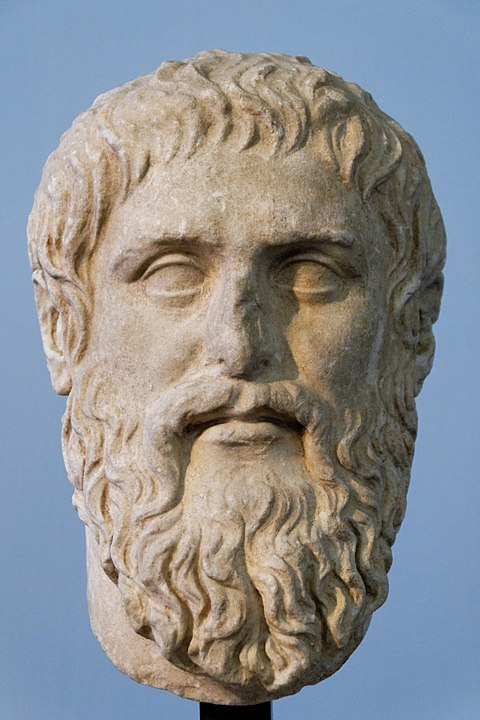
\includegraphics{images/plato_bust.jpg}

		% 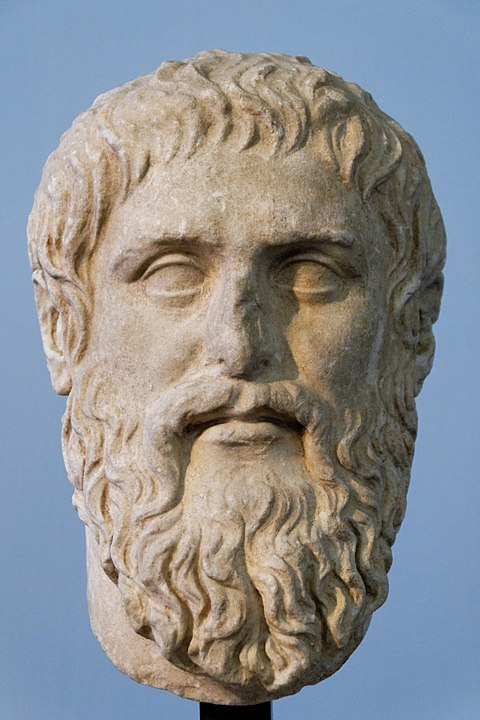
\includegraphics[scale=0.5]{images/plato_bust.jpg}

		% 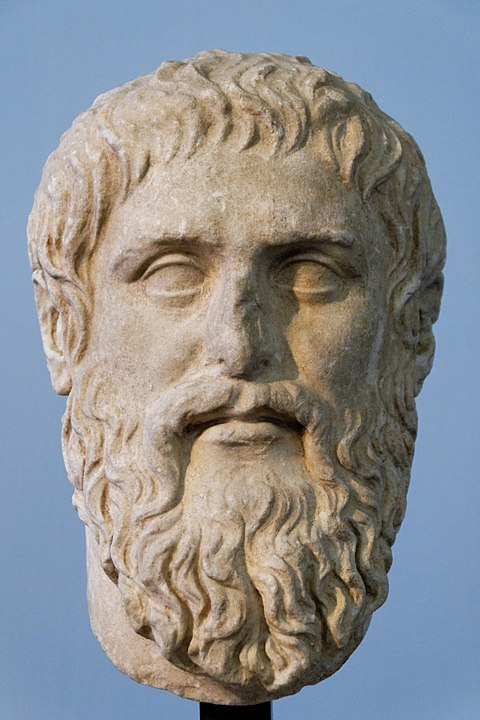
\includegraphics[width=0.3\textwidth, keepaspectratio]{images/plato_bust.jpg}

		\begin{figure}[ht]
			\centering
			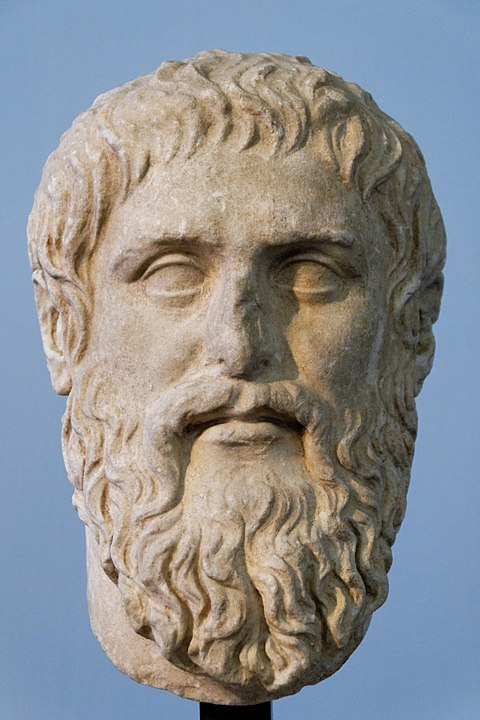
\includegraphics[width=0.3\textwidth, keepaspectratio]{images/plato_bust.jpg}
			\caption{Plato's potrait bust}
			\label{img:platobust}
		\end{figure}

		% remove wiki references - search and replace - \[\d*\]

		%The specific birthdate of Plato is not known. Based on ancient sources, most modern scholars estimate that Plato was born between 428 and 427 BC. The grammarian Apollodorus of Athens argues in his Chronicles that Plato was born in the first year of the eighty-eighth Olympiad (427 BC), on the seventh day of the month Thargelion; according to this tradition the god Apollo was born this day.[2] According to another biographer of him, Neanthes, Plato was eighty-four years of age at his death.[3] If we accept Neanthes' version, Plato was younger than Isocrates by six years, and therefore he was born in the second year of the 87th Olympiad, the year Pericles died (429 BC).[4]
		%The Chronicle of Eusebius names the fourth year of the 89th Olympiad as Plato's, when Stratocles was archon, while the Alexandrian Chronicle mentions the eighty-ninth Olympiad, in the archonship of Isarchus.[5] According to Suda, Plato was born in Aegina in the 88th Olympiad amid the preliminaries of the Peloponnesian war, and he lived 82 years.[6] Sir Thomas Browne also believes that Plato was born in the 88th Olympiad.[7] Renaissance Platonists celebrated Plato's birth on November 7.[8] Ulrich von Wilamowitz-Moellendorff estimates that Plato was born when Diotimos was archon eponymous, namely between July 29 428 BC and July 24 427 BC.[9] Greek philologist Ioannis Kalitsounakis believes that the philosopher was born on May 26 or 27, 427 BC, while Jonathan Barnes regards 428 BC as year of Plato's birth.[10] For her part, Debra Nails asserts that the philosopher was born in 424/423 BC.[8]
		%Plato's birthplace is also disputed. Diogenes Laërtius states that Plato "was born, according to some writers, in Aegina in the house of Phidiades the son of Thales". Diogenes mentions as one of his sources the Universal History of Favorinus. According to Favorinus, Ariston and his family were sent by Athens to settle as cleruchs (colonists retaining their Athenian citizenship), on the island of Aegina, from which they were expelled by the Spartans after Plato's birth there.[3] Nails points out, however, that there is no record of any Spartan expulsion of Athenians from Aegina between 431 and 411 BC.[11] On the other hand, at the Peace of Nicias, Aegina was silently left un der Athens control, and it was not until the summer of 411 that the Spartans overran the island.[12] Therefore, Nails concludes that "perhaps Ariston was a cleruch, perhaps he went to Aegina in 431, and perhaps Plato was born on Aegina, but none of this enables a precise dating of Ariston's death (or Plato's birth)".[11] Aegina is regarded as Plato's place of birth by Suda as well.[6]

		\subsection{Plato's Birth}
			\subsubsection{Plato's birthdate is not known}
				The specific birthdate of Plato is not known. Based on ancient sources, most modern scholars estimate that Plato was born between 428 and 427 BC. The grammarian Apollodorus of Athens argues in his Chronicles that Plato was born in the first year of the eighty-eighth Olympiad (427 BC), on the seventh day of the month Thargelion; according to this tradition the god Apollo was born this day. According to another biographer of him, Neanthes, Plato was eighty-four years of age at his death. If we accept Neanthes' version, Plato was younger than Isocrates by six years, and therefore he was born in the second year of the 87th Olympiad, the year Pericles died (429 BC).

				The Chronicle of Eusebius names the fourth year of the 89th Olympiad as Plato's, when Stratocles was archon, while the Alexandrian Chronicle mentions the eighty-ninth Olympiad, in the archonship of Isarchus. According to Suda, Plato was born in Aegina in the 88th Olympiad amid the preliminaries of the Peloponnesian war, and he lived 82 years. Sir Thomas Browne also believes that Plato was born in the 88th Olympiad. Renaissance Platonists celebrated Plato's birth on November 7. Ulrich von Wilamowitz-Moellendorff estimates that Plato was born when Diotimos was archon eponymous, namely between July 29 428 BC and July 24 427 BC. Greek philologist Ioannis Kalitsounakis believes that the philosopher was born on May 26 or 27, 427 BC, while Jonathan Barnes regards 428 BC as year of Plato's birth. For her part, Debra Nails asserts that the philosopher was born in 424/423 BC.

			\subsubsection*{Plato's birthplace is unkwown}
				Plato's birthplace is also disputed. Diogenes Laërtius states that Plato ``was born, according to some writers, in Aegina in the house of Phidiades the son of Thales". Diogenes mentions as one of his sources the Universal History of Favorinus. According to Favorinus, Ariston and his family were sent by Athens to settle as cleruchs (colonists retaining their Athenian citizenship), on the island of Aegina, from which they were expelled by the Spartans after Plato's birth there. Nails points out, however, that there is no record of any Spartan expulsion of Athenians from Aegina between 431 and 411 BC. On the other hand, at the Peace of Nicias, Aegina was silently left under Athens control, and it was not until the summer of 411 that the Spartans overran the island. Therefore, Nails concludes that ``perhaps Ariston was a cleruch, perhaps he went to Aegina in 431, and perhaps Plato was born on Aegina, but none of this enables a precise dating of Ariston's death (or Plato's birth)". Aegina is regarded as Plato's place of birth by Suda as well.

	\section{Plato's main interests} %lists
		% Metaphysics Ethics Politics Epistemology Rhetoric Art Literature Education Society Friendship Love
		% macro: qs^ei<CR><Esc>^q
		% What were Plato's main interests in terms of his work...
		What were Plato's main interests in terms of his work \ldots

		\subsection{Unordered and ordered Lists}
			Unordered list:
			\begin{itemize}[label=$\ast$, align=right]
    		  	\item Metaphysics
				\item Ethics
				\item Politics
				\item Epistemology
				\item Rhetoric
				\item Art
				\item Literature
				\item Education
				\item Society
				\item Friendship
				\item Love
			\end{itemize}

			Ordered list:
			% \begin{enumerate}[label={\Alph*.}]
			% \begin{enumerate}[label={\alph*.}]
			% \begin{enumerate}[label={\roman*.}]
			% \begin{enumerate}[label={\Roman*.}]
			% \begin{enumerate}[label={(\greek*)}]

			Unordered list:
			% \begin{itemize}[label={}]

			\begin{enumerate}
    			\item Metaphysics
				\item Ethics
				\item Politics
				\item Epistemology
				\item Rhetoric
				\item Art
				\item Literature
				\item Education
				\item Society
				\item Friendship
				\item Love
			\end{enumerate}

			Inline list: \\
			\begin{enumerate*}
				\item Metaphysics
				\item Ethics
				\item Politics
				\item Epistemology
				\item Rhetoric
				\item Art
				% \item Literature
				\item \mbox{Literature}
				\item Education
				\item Society
				\item Friendship
				\item Love
			\end{enumerate*}

		\subsection{Nested lists}
			% enter nested lists from further plato-wiki-index and further in the forms as concrete and abstract objects
			Nested list:
			\begin{enumerate}
    			\item Metaphysics
					\begin{enumerate}
						\item The forms
							\begin{enumerate}
								\item Concrete
								\item[12.] Abstract
							\end{enumerate}
						\item The soul
					\end{enumerate}
				\item Ethics
				\item Politics
				\item Epistemology
					\begin{enumerate}
						\item Recollection
						\item Justified true belief
					\end{enumerate}
				\item Rhetoric
				\item Art
			\end{enumerate}

		\subsection{\texttt{description} lists}
			\paragraph{Although} these propositions are often identified by Plato's readers as forming a large part of the core of his philosophy, many of his greatest admirers and most careful students point out that few, if any, of his writings can accurately be described as mere advocacy of a cut-and-dried group of propositions. Often Plato's works exhibit a certain degree of dissatisfaction and puzzlement with even those doctrines that are being recommended for our consideration. For example, the forms are sometimes described as hypotheses (see for example Phaedo). The form of good in particular is described as something of a mystery whose real nature is elusive and as yet unknown to anyone at all (Republic). Puzzles are raised---and not overtly answered---about how any of the forms can be known and how we are to talk about them without falling into contradiction (Parmenides), or about what it is to know anything (Theaetetus) or to name anything (Cratylus). When one compares Plato with some of the other philosophers who are often ranked with him---Aristotle, Aquinas, and Kant, for example---he can be recognized to be far more exploratory, incompletely systematic, elusive. 
			\par The most important works of Plato are as follows:
			% \begin{description}[align=right, labelwidth=2cm]
			\begin{description}[align=right]
				\item[Apology] Apology is among the most frequently read of Plato's works. In the Apology, Socrates tries to dismiss rumors that he is a sophist and defends himself against charges of disbelief in the gods and corruption of the young.
				\item[Phaedo] In the Phaedo, the title character lists those who were in attendance at the prison on Socrates' last day, explaining Plato's absence by saying, ``Plato was ill".
				\item[Republic] In the Republic, Socrates explains why an enlightened man (presumably himself) will stumble in a courtroom situation. Plato's support of aristocracy and distrust of democracy is also taken to be partly rooted in a democracy having killed Socrates.
			\end{description}

			\begin{description}[align=left]
				\item[Apology] Apology is among the most frequently read of Plato's works. In the Apology, Socrates tries to dismiss rumors that he is a sophist and defends himself against charges of disbelief in the gods and corruption of the young.
				\item[Phaedo] In the Phaedo, the title character lists those who were in attendance at the prison on Socrates' last day, explaining Plato's absence by saying, ``Plato was ill".
				\item[Republic] In the Republic, Socrates explains why an enlightened man (presumably himself) will stumble in a courtroom situation. Plato's support of aristocracy and distrust of democracy is also taken to be partly rooted in a democracy having killed Socrates.
			\end{description}

	\section{Plato's Mentor}
		Socrates was Plato's mentor. \href{https://classicalwisdom.com/wp-content/uploads/2012/12/plato-socrates.jpg}{Here} is a painting of Socrates and Plato taking a walk.

		Here is the wikipedia page about Socrates: \url{https://en.wikipedia.org/wiki/Socrates}.

		Figure \ref{img:platobust} is a picture of Plato's bust

		\href{run:./images/death_of_socrates.jpg}{Here} is picture of Socrates's death.

		I just read an interesting book\cite{finley1977aspects} about Plato.

	\section{Mumbai's weather}
		\begin{tabular}{c c c}
			1 & 2 & 3 \\
			1 & 2 & 3 \\
			1 & 2 & 3 \\
		\end{tabular}
		% using just tabular - BAD PRACTICE
		
		\subsection{\texttt{table} environment}
			The temperature is 30\si{\celsius} today.
			% using table environment - it makes positioning of tables easy
			\begin{table}[h!]
				\centering	
				\begin{tabular}{ |c|c|c| }
					\hline
					\textbf{Day} & \textbf{Max. Temp} & \textbf{Min. Temp.} \\
					\hline
					Tuesday   & 40\si{\celsius} & 45\si{\celsius} \\
					Wednesday & 20\si{\celsius} & 30\si{\celsius} \\
					Thursday  & 30\si{\celsius} & 60\si{\celsius} \\
					Friday    & 10\si{\celsius} & 20\si{\celsius} \\
					Monday    & 30\si{\celsius} & 40\si{\celsius} \\
					\hline
				\end{tabular}
				\caption{Temperatures in the city of Mumbai.}
				\label{table:temp-mumbai}
			\end{table}

		\subsection{Multi-columns and multi-rows}
			% \multicolumn{4}{|c|}{Combined Row} & Cell42 \\ \hline
			\begin{table}[ht]
				\centering
				\begin{tabular}{*{5}{|c}|}
					\hline
					Blank Space & Column1 & Column2 & Column3 & Column4 \\ \hline
					Row1        & Cell11  & Cell21  & Cell31  & Cell41  \\ \hline
					Row2        & Cell12  & Cell22  & Cell32  & Cell42  \\ \hline
					Row3        & Cell13  & Cell23  & Cell33  & Cell43  \\ \hline
					Row4        & Cell14  & Cell24  & Cell34  & Cell44  \\ \hline
				\end{tabular}
			\end{table}

			% \begin{table}[ht]
			% 	\centering
			% 	\begin{tabular}{*{5}{|c}|}
			% 		\hline
			% 		Blank Space     & Column1                        & Column2 & Column3 & Column4 \\ \hline
			% 		Row1            & \multirow{3}{*}{Multiple rows} & Cell21  & Cell31  & Cell41  \\ \cline{3-5}
			% 		\cline{1-1}Row2 &                                & Cell22  & Cell32  & Cell42  \\ \cline{3-5}
			% 		\cline{1-1}Row3 &                                & Cell23  & Cell33  & Cell43  \\ \hline
			% 		Row4            & Cell14                         & Cell24  & Cell34  & Cell44  \\ \hline
			% 	\end{tabular}
			% \end{table}
	
	\bibliography{refs.bib}
	\bibliographystyle{alpha}

\end{document}
